\begin{figure}[!h]
    \centering
    \caption{Paths in $\Z^2$ 1) of length $1$; 2) of length $k + 1$}
    \label{fig:nb_self_avoiding_path}
    \minipage{0.5\textwidth}
    \centering
    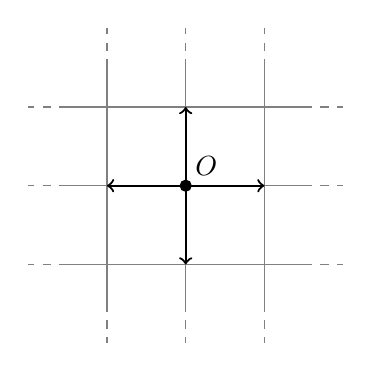
\begin{tikzpicture}
        \foreach \i in {-1, 0, 1} {
            \draw[gray] (-1.5, \i) -- (1.5, \i);
            \draw[gray] (\i, -1.5) -- (\i, 1.5);
            \draw[gray, dashed] (-1.5, \i) -- (-2.0, \i);
            \draw[gray, dashed] (\i, -1.5) -- (\i, -2.0);
            \draw[gray, dashed] (1.5, \i) -- (2.0, \i);
            \draw[gray, dashed] (\i, 1.5) -- (\i, 2.0);
        }
        
        \filldraw (0, 0) circle (2pt);
        \draw[->, thick] (0, 0) -- (1, 0);
        \draw[->, thick] (0, 0) -- (0, 1);
        \draw[->, thick] (0, 0) -- (-1, 0);
        \draw[->, thick] (0, 0) -- (0, -1);
        \node[right] at (0.0, 0.25) {$O$};
    \end{tikzpicture}
    \endminipage\hfill
    % --
    \minipage{0.5\textwidth}
    \centering
    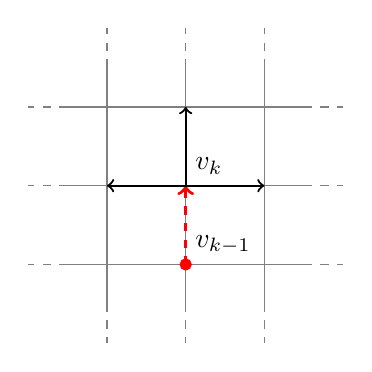
\begin{tikzpicture}
        \foreach \i in {-1, 0, 1} {
            \draw[gray] (-1.5, \i) -- (1.5, \i);
            \draw[gray] (\i, -1.5) -- (\i, 1.5);
            
            \draw[gray, dashed] (-1.5, \i) -- (-2.0, \i);
            \draw[gray, dashed] (\i, -1.5) -- (\i, -2.0);
            \draw[gray, dashed] (1.5, \i) -- (2.0, \i);
            \draw[gray, dashed] (\i, 1.5) -- (\i, 2.0);
        }
        
        \draw[->, red, dashed, very thick] (0, -1) -- (0, 0);
        \filldraw[red] (0, -1) circle (2pt);
        \draw[->, thick] (0, 0) -- (1, 0);
        \draw[->, thick] (0, 0) -- (0, 1);
        \draw[->, thick] (0, 0) -- (-1, 0);
        \node[right] at (0.0, 0.25) {$v_k$};
        \node[right] at (0.0, -0.75) {$v_{k - 1}$};
    \end{tikzpicture}
    \endminipage
\end{figure}